
\chapter{Hybrid approach} 
\label{ch:hybrid}

In this chapter we want to explore some possible combinations of the before mentioned algorithm schemes and then present the main result of this work, the tree-flavored-invariant-polytope-algorithm and its termination results. 

\begin{section}{Goal and options}
In its heart the invariant-polytope algorithm tries to find a polytope, which corrisponding minkowski-norm is specifically optimized on the given problem, whilst the finite-tree algorithm connects growth-rate to decompositions of products. A clear combination scheme arises naturally, where we use the optimized polytope norm to estimate the products of the finite-tree. From there we can choose a specific order or level of concurrency.
\newline
The most modular approach would be to first run the invariant-polytope algorithm for a couple of runs and then use the calculated norm thats specially optimized for the finite-tree algorithm. But that seems to be wasteful since valuable matrix calculations from the finite-tree algorithm could have been used for an even more optimized norm and some polytopes might have already cleared insight for the decompositions that the finite-tree algorithm tries to find. In \citep{mejstrikHybridApproachJoint} the authors came up with a more concurrent algorithm that builds up norms and decompositions in every step. 
\end{section}

\section{Structure of the hybrid algorithm}

We try to decompose arbitrary products $P \in \mathcal{A}^k$, such that their polytope-norms are less then $p(k)$ where $p$ is a monotone polynomial.
This removes the invariance property of the polytope to be build up, since the norms dont have to be less than 1 but it still proofes the JSR identity because we take the averaged norms in the length of the products in the three-member-inequality ~\ref{eq:three-member}.
\newline 
Starting the loop of the invariant-polytope algorithm with a cycle on top that is connected via the generators factors and also the first branches represented by images from the missing $J-1$ factors from $\mathcal{A}$. Instead of only adding images under vertices from $V$ and matrices from $\mathcal{A}$ directly, from now on we try to find an $(\mathcal{A},\mathbf{G})\text{-tree}$ which is one-bounded i.e its leafage-polytope-norm is less than 1, for every $v \in V$.
For that we generate $(\mathcal{A},\mathbf{G})\text{-tree}$ patterns in the beginning and just go through every remaining vertex and calculate the leafage-norms. From the structure of those trees we can assume that every matrix in $\mathcal{A}$ represents a node for the first branches.
For the branches that lead to a leafage-norm less than or equal 1 we are done, for the other branches we have the choice to go deeper or just add some points to $V$ that changes the leafage-norm of those branches to less than 1. Here we decided to add the points since going deeper just would mean to consider possibly the same products but the tree generation would be more complex with options for depth-first- or breadth-first-search and even using some s.m.p and generator trickery. [might change it in the future]
\newline
First points that come to mind are the leafage-points itself since this is what we have tested but generators could be involved meaning there are possibly infinitely many leafage-points. So the next best thing would be the roots of the branches which are guaranteed to be a single matrix from $\mathcal{A}$. This makes tree generation easy and adds points with likely more distance to the faces of the polytope and makes the norm stronger more quickly.
\newline
So in principle for every $v \in V_{\text{rem}}$ take a tree from the generating pool, check the leafage-norm for every root branch, if it is larger than 1 add the point from the root branch to $V_{\text{new}}$ and $V$. Repeat this as long as new vertices have been added. We use $V$ for the polytope-norms and since new points are only being added the norms decrease over time so all 1-bounded trees stay bounded.
\newline
After termination the set of trees generated promise a valid decomposition for every product from $\mathcal{A}$ into chunks of norm lesser 1 and one suffix thats of norm less than $p(k)$ for some monotone polynomial, which proofes the question if the chosen radius is maximal.

\vspace{1cm}

\begin{algorithm}
  \caption{Tree-flavored-invariant-polytope-algorithm}
  \label{alg:hybrid}
  \begin{algorithmic}
      \State $V := \{v_1, \cdots, v_M\}$
      \State $V_{\text{new}} \gets V$
      \While {$V_{\text{new}} \ne \emptyset$}
          \State $V_{\text{rem}} \gets V_{\text{new}}$
          \State $V_{\text{new}} \gets \emptyset$
          \For {$v \in V_{\text{rem}}$}
              \State $\text{Construct some } (\mathcal{A},\mathbf{G})\text{-tree } \mathbf{T}$
              \For {$L = L'A \in \mathcal{L}(T) \text{ with } A \in \mathcal{A}$}
                  \If {$\lVert Lv \rVert _{\text{co}_{\text{s}}(V)} \geq 1$}
                      \State $V Av$
                      \State $V_{\text{new}} \gets V_{\text{new}} \cup Av$
                  \EndIf
              \EndFor
          \EndFor
      \EndWhile \\
      \Return \\
  \end{algorithmic}
\end{algorithm}

\vspace{1cm}

The following figure~\ref{fig:cyclic_tree_structure} shows an example of the generated tree structure as well as the tested $(\mathcal{A},\mathbf{G})\text{-trees}$ that have been used to bound the products. Here $\mathcal{A}$ consists of two matrices $A$ and $B$ and the chosen candidate is $ \Pi = ABA$. At the top you can see the cycle generated by the candidate and the starting vector $v_1$ as well as branches coming of, that are the products that stay in contrast to the cycle. This is what i call the crown and it is generated for every matrix set at the beginning, so no testing has been made so far. All the nodes that are connected through a solid arrow have been added to the vertices $V$.

\begin{figure}[H]
  \centering
  \begin{tikzpicture}[
    edge from parent/.style={draw, -latex, dashed, thick},
    level distance=10mm,
    sibling distance=23mm
  ]
  
  % Cycle 
  \node (v1) at (-1.5, 2) {$v_1$};
  \node (v2) at (1.5, 2) {$v_2$};
  \node (v3) at (0, 0) {$v_3$};
  
  \draw[-latex, thick, bend left=30] (v1) to node[midway, above] {$A$} (v2);
  \draw[-latex, thick, bend left=30] (v2) to node[midway, above] {$B$} (v3);
  \draw[-latex, thick, bend left=30] (v3) to node[midway, above] {$A$} (v1);
  
  % Left side 
  \node (v4) at (-3.5,0) {$v_4$}
    child[grow=-130, level distance=15mm]{node{$\{Av_4\}$}}
    child[grow=-50, level distance=15mm]{node{$\{Bv_4\}$}};

  \draw[-latex, thick, rounded corners] (v1) to node[midway, above] {$B$} (v4);

  % Right side
  \node (v5) at (4,-0.5) {$v_5$}
    child {node {$\{ Av_7\}$}}
    child {
      child {
        child {node {$\{AG^nBv_5\}$}} 
        child {
          child {node {$\{ABG^nBv_5\}$}} 
          child {node {$\{BBG^nBv_5\}$}}
        }
      }
    };

  % Add G label to generator branch
  \node[right] at (4.5,-2) {$G$};

  \draw[-latex, thick] (v2) to node[midway, above] {$A$} (v5);
  
  % Middle with adjusted growth angle for v6 subtree
  \node (v6) at (-0.5,-1.5) {$v_6$}
    child[grow= -140, level distance=20mm] { 
      node (v7) {$v_7$}  
      child[grow= -140, level distance=15mm] {node {$\{ Av_7\}$}}
      child[grow= -55, level distance=10mm] {
        child[grow= -90] { 
          child {node {$\{AG^nBv_7\}$}} 
          child {node {$\{BG^nBv_7\}$}}
        }
      }
    }
    child {
      child[grow=-135, level distance=11mm] {node {$\{ ABv_6\}$}}
      child[grow=-45, level distance=11mm] {node {$\{ BBv_6\}$}}
    };

  \draw[-latex, thick, rounded corners] (v3) to node[right, pos=0.5] {$B$} (v6);
  
  % Override the edge from v6 to v7 with longer length and consistent arrow style
  \draw[-latex, thick] (v6) -- ($(v6)!0.78!(v7)$);
  \node[above] at ($(v6)!0.5!(v7)$) {$A$};
  \node[above] at ($(v6)!0.6!(v6-2)$) {$B$};
  
  \end{tikzpicture}
  \caption{Cyclic tree structure generated by the algorithm. Vertices added to $V$ (solid arrows) and finite-trees for bounding products (dashed arrows).}
  \label{fig:cyclic_tree_structure}
\end{figure}

Now the finite-tree theory comes in and every vertex gets tested by a $(\mathcal{A},\mathbf{G})\text{-tree}$ (dashed arrows). Take the vector $v_6$ for example it has been tested by an tree and the branch starting with the matrix $B$ was sufficient i.e. every leaf-node has a polytope-norm of less than 1 (at the time the polytope consists of the vertices $V = \{v_1, \cdots, v_6\}$). The branch starting with the matrix $A$ on the other hand did not, so the vertex $v_7 = Av_6$ has been added to $V$ and the next tree was tested, which was fully sufficient (on every branch). Since the other branches also terminated earlier the algorithm stops, no more vertices are beeing added and the candidate $\Pi$ was proofen to be a s.m.p product. 

\section{Termination results}

\begin{lemma}
  \label{lem:poly}
  For every cyclic-tree $T$ generated by algortihm \ref{alg:hybrid}, there exists a monotone polynomial $p$ that bounds every product $P$ encoded by nodes of the tree in the produced polytope-norm and according to the length $\lvert P \rvert$ of the product (number of used factors from $\mathcal{A}$): 
  $$
    \exists p: \forall P \in T: \lVert P \rVert _{V} \le p(\lvert P \rvert)
  $$
\end{lemma}

\begin{proof}
  Take an arbitrary node $N = [i_1, \cdots, i_n]$ of the generated tree. 
  Now every $i_j$ encodes either a matrix from $\mathcal{A}$ or a generator from $\mathcal{G}$. 
  Since all those matrices have a spectral radius less then 1, its Jordan-Normal forms grow utmost polynomially und thus, due to equality of norms in finite-dimensional vector spaces, we have that $ \exists p_{i_j}: \lVert A_{i_j} \rVert _V \le p_{i_j}(\lvert A_{i_j} \rvert)$, where the number of factors only matters for generators since they are encoded for any exponent $n \in \N$.
  Here $ A_{i_j} $ stand for the actual factors from an arbitrary product encoded by $N$ so that $\lvert A_{i_j} \rvert$ is well defined. 
  Now we take the product of those polynomials and get an upper bound for every product encoded by this node. 

  $$ 
    \text{Let:} \quad k = \sum \limits_{j = 1}^{n} \lvert A_{i_j} \rvert \quad \text{and} \quad p_{N} = \prod \limits_{j = 1}^{n} p_{i_j}
  $$
  $$ 
    \lVert A_{i_n} \cdot ... \cdot A_{i_1} \rVert _V \le \lVert A_{i_n} \rVert _V \cdot ... \cdot \lVert A_{i_1} \rVert _V \le p_{i_n}(\lvert A_{i_n} \rvert) \cdot ... \cdot p_{i_1}(\lvert A_{i_1} \rvert)
  $$
  $$
    \le p_{i_n}(k) \cdot ... \cdot p_{i_1}(k) = p_{N}(k)
  $$
  So since the node was arbitrary we have such a polynomial $p_N$ for every node $N \in T$. 
  
  $$
    \text{Now let } \quad p_N = \sum \limits_{r \geq 0} \lambda_{N,r} x^r \quad \text{then} \quad p = \sum \limits_{r \geq 0} \max \limits_{N \in T}\lambda_{N,r}x^r
  $$
  and due to the fact that the tree has only finitely many nodes, the maximum is actually well defined. This concludes the lemma.
  
\end{proof}

\begin{lemma}
  \label{lem:arb.prod.bound}
  There exists an monotone polynomial $p$ such that for every product $P \in \mathcal{A}^k$ and $v \in V$, $\lVert Pv \rVert _V \le p(k)$ holds.
\end{lemma}

\begin{proof}
  Since for every $v \in V$ there exists an $(\mathcal{A},\mathbf{G})\text{-tree}$ that is 1-bounded, we can find a leaf $L$ and according suffix $P'$ such that $P = P'L$ and $Lv = \sum _{i=1}^{J} \lambda _{i} v_{i}$ with $\sum _{i=1}^{J} |\lambda _{i} |\leq 1$. \\
  Now we have: 
  \begin{equation*}
  \| Pv\| _{V} =\| P'Lv\| _{V} \ =\ \| P'\sum _{i=1}^{J} \lambda _{i} v_{i} \| _{V} \leq \sum _{i=1}^{J} |\lambda _{i} |\| P'v_{i} \| _{V}
  \end{equation*}
  This means we got to the same point as the beginnig in bounding the product of an arbitrary $P'$ and $v \in V$. Since the leafs of an $(\mathcal{A},\mathbf{G})\text{-tree}$ have always one or more factors, the sice of $P'$ decreased from the sice of $P$. So if we repeat the process enough times $P'$ lies within the tree $T$ and therefore, according to lemma \ref{lem:poly}, there exists a monotone polynomial $p$ such that: $$\|P'\| _{V} \leq p(|P'|) \leq p(|P|)$$
  This implies:
  \begin{equation*}
  \| Pv\| _{V} \leq \sum _{i=1}^{J} |\lambda _{i} |\| P'v_{i} \| _{V} \leq \sum _{i=1}^{J} |\lambda _{i} |\| P'\| _{V} \leq \sum _{i=1}^{J} |\lambda _{i} |p( |P|) \leq p( |P|)
  \end{equation*}
  Which concludes the proof.
\end{proof}

\begin{theorem}{}\label{thm:hybrid-found}
If Algorithm~\ref{alg:hybrid} terminates then $JSR(\mathcal{A}) \leq 1$
\end{theorem}

\begin{proof}
  Due to the prework in the lemmas this is now easy to show. 
  Lemma \ref{lem:arb.prod.bound} implies that for every $P \in \mathcal{A}^k$ and $v \in V$, $\lVert Pv \rVert _V \le p(k)$
  trivially this implies: 
  $$
    \forall P \in \mathcal{A}^k: \lVert P \rVert _V \le p(k)
  $$
  Now we take the definition of the $JSR$ and get:
  $$
    JSR(\mathcal{A}) = \lim_{k \geq 1} \max_{P \in \mathcal{A}^k} \lVert P \rVert^\frac{1}{k} \le \lim_{k \geq 1} p(k)^\frac{1}{k} = 1
  $$ 
\end{proof}

Of course, if the candidate had a spectral radius of $1 \implies JSR(\mathcal{A}) = 1$.

\begin{corollary}
  If the chosen trees are always $T_v = \mathcal{A}$, then we would have exactly the invariant-polytope algorithm \ref{alg:exact}. 
  Which makes the new approach a real generalization. \\
  Also the polynomial bounding would collapse to just a constant $ K = \max\limits_{v \in V}\max\limits_{P \in T_{v}}: \lVert P \rVert _{co_{s}(V)}$ that is the maximum over all polytope-norm values of nodes in the generated cyclic-tree. This constant would not depend on the sizes of the products anymore.
\end{corollary}

\section{Efficiency}

\subsection*{Remarks}
\subsubsection*{Used trees}
It was proofen in \citep{mollerTreebasedApproachJoint2014} that in order to have a bigger solution space then algorithm \ref{alg:exact} the use of generators is mandatory. 
The choice of the testing-trees is not trivial and subject to active research. 
We propose to use so-called minimal trees that fulfill every necessary and beneficial condition of the $(\mathcal{A},\mathbf{G})\text{-trees}$ but keep the amount of nodes minimal.

\subsubsection*{Stopping criterions}
Some of the stopping criterions of the invariant-polytope algorithm can still be used as the structure is very similar. 
For this the eigenplane stopping condition is implemented. 

\subsubsection*{Polytope invariance}
Since the polytope-norms of matrices in $\mathcal{A}$ are allowed to be bigger than 1 just less than $p(1)$ it is possible and very likely the polytope is not invariant.

\subsection{Implementation}

\begin{definition}
  An $(\mathcal{A},\mathbf{G})\text{-tree}$ with just one generator at the root, one path from root to the covered node and all neccessarily added branches, to make it comply with definition~\ref{def:tree}, is called a \emph{minimal tree}. This tree only depends on the set $\mathcal{A}$ and the chosen generator $G$. Its denoted by $\min(G, \mathcal{A})$.
\end{definition}

\tikzset{every picture/.style={line width=0.75pt}} %set default line width to 0.75pt        

\begin{figure}[!h]
  \centering
  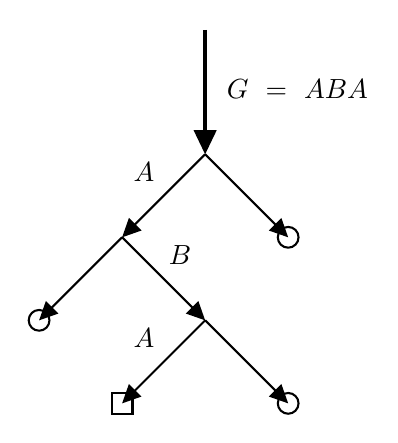
\begin{tikzpicture}[x=0.75pt,y=0.75pt,yscale=-1,xscale=1]
    %uncomment if require: \path (0,477); %set diagram left start at 0, and has height of 477
    
    %Straight Lines [id:da16898060564023787] 
    \draw [line width=1.5]    (300,60) -- (300,116) ;
    \draw [shift={(300,120)}, rotate = 270] [fill={rgb, 255:red, 0; green, 0; blue, 0 }  ][line width=0.08]  [draw opacity=0] (11.61,-5.58) -- (0,0) -- (11.61,5.58) -- cycle    ;
    %Straight Lines [id:da06600633985452076] 
    \draw [line width=0.75]    (300,120) -- (262.12,157.88) ;
    \draw [shift={(260,160)}, rotate = 315] [fill={rgb, 255:red, 0; green, 0; blue, 0 }  ][line width=0.08]  [draw opacity=0] (8.93,-4.29) -- (0,0) -- (8.93,4.29) -- cycle    ;
    %Straight Lines [id:da7450241120277035] 
    \draw    (300,120) -- (337.88,157.88) ;
    \draw [shift={(340,160)}, rotate = 225] [fill={rgb, 255:red, 0; green, 0; blue, 0 }  ][line width=0.08]  [draw opacity=0] (8.93,-4.29) -- (0,0) -- (8.93,4.29) -- cycle    ;
    %Straight Lines [id:da20701336800849934] 
    \draw [line width=0.75]    (260,160) -- (297.88,197.88) ;
    \draw [shift={(300,200)}, rotate = 225] [fill={rgb, 255:red, 0; green, 0; blue, 0 }  ][line width=0.08]  [draw opacity=0] (8.93,-4.29) -- (0,0) -- (8.93,4.29) -- cycle    ;
    %Straight Lines [id:da9104391839581025] 
    \draw [line width=0.75]    (300,200) -- (262.12,237.88) ;
    \draw [shift={(260,240)}, rotate = 315] [fill={rgb, 255:red, 0; green, 0; blue, 0 }  ][line width=0.08]  [draw opacity=0] (8.93,-4.29) -- (0,0) -- (8.93,4.29) -- cycle    ;
    %Straight Lines [id:da14256048753952277] 
    \draw    (260,160) -- (222.12,197.88) ;
    \draw [shift={(220,200)}, rotate = 315] [fill={rgb, 255:red, 0; green, 0; blue, 0 }  ][line width=0.08]  [draw opacity=0] (8.93,-4.29) -- (0,0) -- (8.93,4.29) -- cycle    ;
    %Straight Lines [id:da285744534909546] 
    \draw    (300,200) -- (337.88,237.88) ;
    \draw [shift={(340,240)}, rotate = 225] [fill={rgb, 255:red, 0; green, 0; blue, 0 }  ][line width=0.08]  [draw opacity=0] (8.93,-4.29) -- (0,0) -- (8.93,4.29) -- cycle    ;
    %Shape: Square [id:dp22230762253177927] 
    \draw   (255,235) -- (265,235) -- (265,245) -- (255,245) -- cycle ;
    %Shape: Circle [id:dp7008956868229022] 
    \draw   (335,240) .. controls (335,237.24) and (337.24,235) .. (340,235) .. controls (342.76,235) and (345,237.24) .. (345,240) .. controls (345,242.76) and (342.76,245) .. (340,245) .. controls (337.24,245) and (335,242.76) .. (335,240) -- cycle ;
    %Shape: Circle [id:dp8387416622961836] 
    \draw   (335,160) .. controls (335,157.24) and (337.24,155) .. (340,155) .. controls (342.76,155) and (345,157.24) .. (345,160) .. controls (345,162.76) and (342.76,165) .. (340,165) .. controls (337.24,165) and (335,162.76) .. (335,160) -- cycle ;
    %Shape: Circle [id:dp030752111549602335] 
    \draw   (215,200) .. controls (215,197.24) and (217.24,195) .. (220,195) .. controls (222.76,195) and (225,197.24) .. (225,200) .. controls (225,202.76) and (222.76,205) .. (220,205) .. controls (217.24,205) and (215,202.76) .. (215,200) -- cycle ;
    
    % Text Node
    \draw (309,82.4) node [anchor=north west][inner sep=0.75pt]    {$G\ =\ ABA$};
    % Text Node
    \draw (264,122.4) node [anchor=north west][inner sep=0.75pt]    {$A$};
    % Text Node
    \draw (281,162.4) node [anchor=north west][inner sep=0.75pt]    {$B$};
    % Text Node
    \draw (264,202.4) node [anchor=north west][inner sep=0.75pt]    {$A$};
    
    \end{tikzpicture}
    \caption{Minimal tree structure $\min(G, \mathcal{A})$ for the candidate $G = ABA$ and $\mathcal{A} = \{A,B\}$. The arrows marked with circles are uncovered-leafs, the arrow marked with a square is a covered-leaf}
\end{figure}
